\documentclass[11pt]{article}
\usepackage[margin=2.5cm]{geometry}
\usepackage{booktabs}
\usepackage{graphicx}
\usepackage[hidelinks]{hyperref}
\usepackage{times}
\usepackage{enumitem}
\usepackage{float}
\usepackage{amsmath}
\usepackage{tikz}
\usetikzlibrary{positioning, arrows.meta, calc}
\tikzset{
  nblue/.style={circle, draw=blue!70!black, fill=blue!40, minimum size=5mm, inner sep=0},
  norange/.style={circle, draw=orange!80!black, fill=orange!50, minimum size=5mm, inner sep=0},
  ngreen/.style={circle, draw=green!50!black, fill=green!40, minimum size=5mm, inner sep=0},
  ngray/.style={circle, draw=gray, fill=gray!20, minimum size=5mm, inner sep=0},
  nboth/.style={circle, draw=black, left color=blue!40, right color=orange!50, minimum size=5mm, inner sep=0},
  hub/.style={rectangle, rounded corners=2pt, draw=black, thick, fill=yellow!40, minimum size=6mm, inner sep=1pt, font=\scriptsize\bfseries},
  gedge/.style={gray!70, thick},
  cedge/.style={red!70!black, thick, dashed},
  hedge/.style={black!60, thin},
  hhedge/.style={purple!80!black, very thick},
  ftitle/.style={font=\small\bfseries},
  fnote/.style={font=\footnotesize, align=center}}

\title{Run 4: Clique Ideas and Hub Links}
\author{}
\date{October 27, 2026}

\begin{document}
\maketitle

\section*{What we tested}

Our model is a relational GNN: it keeps separate weights for each type of edge. There are two
edge types. The first is the dataset's own graph. The second ties the nodes of one subgraph
together, in one of two ways (Figure~\ref{fig:setup}):
\begin{itemize}[itemsep=1pt]
  \item \textbf{Clique}: an edge between every two nodes of the same subgraph.
  \item \textbf{Extra node} (hub): one new node per subgraph, linked to all its members. The
        hub's vector is the subgraph's vector.
\end{itemize}

\begin{figure}[H]
\centering
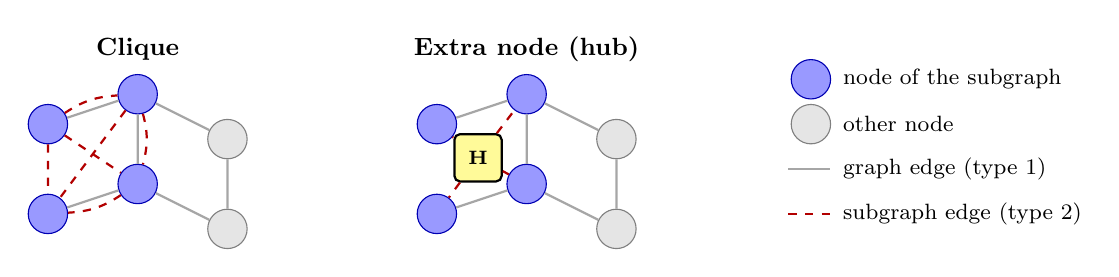
\begin{tikzpicture}[scale=0.95]
  \begin{scope}
    \node[ftitle] at (1.2,2.6) {Clique};
    \node[nblue] (a) at (0,1.6) {};
    \node[nblue] (b) at (1.2,2.0) {};
    \node[nblue] (c) at (1.2,0.8) {};
    \node[nblue] (d) at (0,0.4) {};
    \node[ngray] (e) at (2.4,1.4) {};
    \node[ngray] (f) at (2.4,0.2) {};
    \draw[gedge] (a)--(b) (b)--(c) (c)--(d) (b)--(e) (c)--(f) (e)--(f);
    \draw[cedge] (a)--(c) (a)--(d) (b)--(d) (a) to[bend left=15] (b) (b) to[bend left=15] (c) (c) to[bend left=15] (d);
  \end{scope}
  \begin{scope}[xshift=5.2cm]
    \node[ftitle] at (1.2,2.6) {Extra node (hub)};
    \node[nblue] (a) at (0,1.6) {};
    \node[nblue] (b) at (1.2,2.0) {};
    \node[nblue] (c) at (1.2,0.8) {};
    \node[nblue] (d) at (0,0.4) {};
    \node[ngray] (e) at (2.4,1.4) {};
    \node[ngray] (f) at (2.4,0.2) {};
    \node[hub] (h) at (0.55,1.15) {H};
    \draw[gedge] (a)--(b) (b)--(c) (c)--(d) (b)--(e) (c)--(f) (e)--(f);
    \draw[cedge] (h)--(a) (h)--(b) (h)--(c) (h)--(d);
  \end{scope}
  \begin{scope}[xshift=10.2cm, yshift=0.4cm]
    \node[nblue] at (0,1.8) {}; \node[anchor=west, font=\footnotesize] at (0.3,1.8) {node of the subgraph};
    \node[ngray] at (0,1.2) {}; \node[anchor=west, font=\footnotesize] at (0.3,1.2) {other node};
    \draw[gedge] (-0.3,0.6)--(0.25,0.6); \node[anchor=west, font=\footnotesize] at (0.3,0.6) {graph edge (type 1)};
    \draw[cedge] (-0.3,0.0)--(0.25,0.0); \node[anchor=west, font=\footnotesize] at (0.3,0.0) {subgraph edge (type 2)};
  \end{scope}
\end{tikzpicture}
\caption{The two kinds of subgraph edge, on one subgraph of four nodes.}
\label{fig:setup}
\end{figure}

The advisor's concern (October 23) was that both kinds pull all nodes of a subgraph to one
shared vector, which is close to plain mean pooling, and that this gets worse for big subgraphs.
This run tests the advisor's suggestions and one idea from SubGNN:

\begin{description}[leftmargin=0pt, labelwidth=0pt, itemsep=3pt, font=\normalfont\bfseries]
  \item[No clique.] Graph edges only. Shows what the graph alone gives.
  \item[Clique, symmetric.] Today each node takes the plain mean of its clique neighbors. Here
        the message from node $j$ to node $i$ is divided by $\sqrt{d_i d_j}$ instead, where $d$
        is the number of clique neighbors (as in the original GCN).
  \item[Clique, symmetric $+$ $1/N_C$.] As above, and each clique edge of subgraph $C$ is also
        multiplied by $1/N_C$, where $N_C$ is the number of nodes in $C$. (With a plain mean the
        $1/N_C$ would cancel out, so it is only tried on top of the symmetric version.)
  \item[Hub graph.] The extra-node model, plus a third edge type that links hubs of related
        subgraphs, so a subgraph also hears from other subgraphs (Figure~\ref{fig:hubs}).
\end{description}

\begin{figure}[H]
\centering
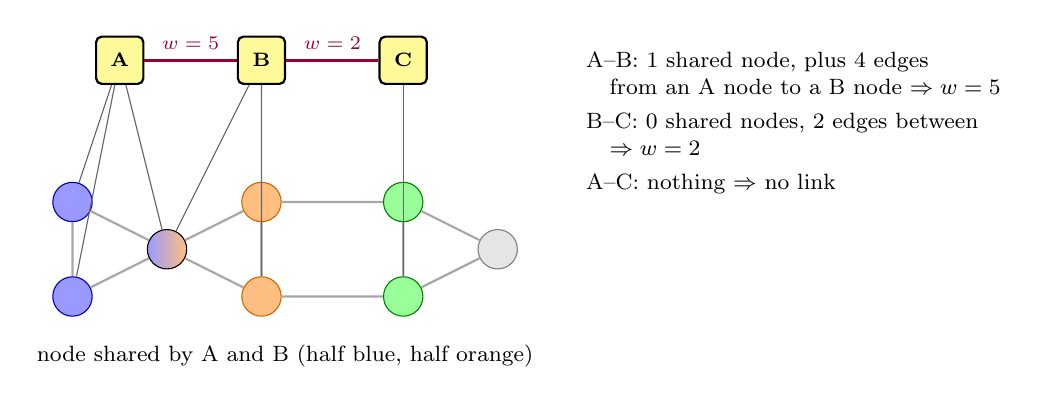
\begin{tikzpicture}[scale=1.0]
  \node[nblue]   (a1) at (0,1.6) {};
  \node[nblue]   (a2) at (0,0.4) {};
  \node[nboth]   (s)  at (1.2,1.0) {};
  \node[norange] (b1) at (2.4,1.6) {};
  \node[norange] (b2) at (2.4,0.4) {};
  \node[ngreen]  (c1) at (4.2,1.6) {};
  \node[ngreen]  (c2) at (4.2,0.4) {};
  \node[ngray]   (g)  at (5.4,1.0) {};
  \draw[gedge] (a1)--(a2) (a1)--(s) (a2)--(s) (s)--(b1) (s)--(b2) (b1)--(b2)
               (b1)--(c1) (b2)--(c2) (c1)--(c2) (c1)--(g) (c2)--(g);
  \node[fnote] at (2.7,-0.35) {node shared by A and B (half blue, half orange)};
  \node[hub] (HA) at (0.6,3.4) {A};
  \node[hub] (HB) at (2.4,3.4) {B};
  \node[hub] (HC) at (4.2,3.4) {C};
  \draw[hhedge] (HA) -- node[above, font=\scriptsize]{$w=5$} (HB);
  \draw[hhedge] (HB) -- node[above, font=\scriptsize]{$w=2$} (HC);
  \draw[hedge] (HA)--(a1) (HA)--(a2) (HA)--(s);
  \draw[hedge] (HB)--(s) (HB)--(b1) (HB)--(b2);
  \draw[hedge] (HC)--(c1) (HC)--(c2);
  \node[anchor=west, font=\footnotesize, align=left] at (6.4,2.6)
    {A--B: 1 shared node, plus 4 edges\\ \quad from an A node to a B node $\Rightarrow w=5$\\[3pt]
     B--C: 0 shared nodes, 2 edges between\\ \quad $\Rightarrow w=2$\\[3pt]
     A--C: nothing $\Rightarrow$ no link};
\end{tikzpicture}
\caption{Hub links (purple). The weight $w$ of a link is the number of nodes the two subgraphs
share plus the number of graph edges between them. Linking every related pair would make the
hubs almost a full clique on most datasets, so each hub keeps only its 10 strongest links.}
\label{fig:hubs}
\end{figure}

Every case starts from the best settings found for the plain clique (run 2), changes only what
the case is about, searches a few learning rates, and then trains 10 seeds. The plain clique was
also trained again with 10 new seeds. em\_user was left out, as before.

\section*{Results}

\begin{table}[H]
\centering
\footnotesize
\setlength{\tabcolsep}{3pt}
\begin{tabular}{lcccc|cc|ccc}
\toprule
 & \multicolumn{4}{c|}{clique models} & \multicolumn{2}{c|}{extra-node models} & \multicolumn{3}{c}{published} \\
dataset & plain & none & symmetric & sym.\ $+1/N_C$ & extra node & hub graph & SubGNN & GLASS & GPEN \\
\midrule
ppi\_bp    & 59.2\,{\scriptsize$\pm$1.1} & 59.9\,{\scriptsize$\pm$2.1} & \textbf{60.0}\,{\scriptsize$\pm$1.9} & 59.4\,{\scriptsize$\pm$2.9} & \textbf{60.6}\,{\scriptsize$\pm$1.9} & 60.3\,{\scriptsize$\pm$1.8} & 59.9\,{\scriptsize$\pm$2.5} & 61.9\,{\scriptsize$\pm$2.2} & \textbf{64.4}\,{\scriptsize$\pm$0.9} \\
hpo\_metab & 54.7\,{\scriptsize$\pm$3.4} & 53.7\,{\scriptsize$\pm$2.8} & \textbf{55.3}\,{\scriptsize$\pm$2.4} & 53.7\,{\scriptsize$\pm$3.3} & 52.4\,{\scriptsize$\pm$4.3} & \textbf{52.6}\,{\scriptsize$\pm$2.3} & 53.7\,{\scriptsize$\pm$2.5} & 61.4\,{\scriptsize$\pm$1.6} & \textbf{63.9}\,{\scriptsize$\pm$0.9} \\
hpo\_neuro & 62.4\,{\scriptsize$\pm$0.9} & 62.7\,{\scriptsize$\pm$1.0} & \textbf{63.2}\,{\scriptsize$\pm$1.1} & 63.0\,{\scriptsize$\pm$1.6} & \textbf{60.9}\,{\scriptsize$\pm$1.2} & 60.3\,{\scriptsize$\pm$0.9} & 64.4\,{\scriptsize$\pm$1.9} & 68.5\,{\scriptsize$\pm$1.6} & \textbf{69.1}\,{\scriptsize$\pm$0.6} \\
density    & \textbf{78.8}\,{\scriptsize$\pm$6.5} & 70.8\,{\scriptsize$\pm$3.1} & 75.2\,{\scriptsize$\pm$4.7} & 72.8\,{\scriptsize$\pm$3.9} & 67.2\,{\scriptsize$\pm$5.0} & \textbf{69.2}\,{\scriptsize$\pm$5.4} & 91.9\,{\scriptsize$\pm$1.9} & 93.0\,{\scriptsize$\pm$2.8} & \textbf{95.6}\,{\scriptsize$\pm$1.6} \\
cut\_ratio & \textbf{75.6}\,{\scriptsize$\pm$4.9} & 73.2\,{\scriptsize$\pm$3.6} & 73.2\,{\scriptsize$\pm$4.0} & \textbf{75.6}\,{\scriptsize$\pm$3.3} & 79.2\,{\scriptsize$\pm$3.0} & \textbf{81.6}\,{\scriptsize$\pm$2.7} & 62.9\,{\scriptsize$\pm$4.1} & 93.5\,{\scriptsize$\pm$1.9} & \textbf{93.6}\,{\scriptsize$\pm$1.6} \\
coreness   & 84.4\,{\scriptsize$\pm$5.2} & 82.6\,{\scriptsize$\pm$3.4} & 84.4\,{\scriptsize$\pm$5.2} & \textbf{84.8}\,{\scriptsize$\pm$4.9} & 76.5\,{\scriptsize$\pm$3.5} & \textbf{78.7}\,{\scriptsize$\pm$3.1} & 65.9\,{\scriptsize$\pm$9.8} & 84.0\,{\scriptsize$\pm$2.8} & \textbf{87.6}\,{\scriptsize$\pm$1.9} \\
component  & \textbf{99.2}\,{\scriptsize$\pm$1.6} & 86.0\,{\scriptsize$\pm$12.2} & 84.8\,{\scriptsize$\pm$21.5} & 83.2\,{\scriptsize$\pm$23.2} & 67.2\,{\scriptsize$\pm$8.5} & \textbf{92.0}\,{\scriptsize$\pm$3.6} & 95.8\,{\scriptsize$\pm$10.1} & \textbf{100.0}\,{\scriptsize$\pm$0.0} & \textbf{100.0}\,{\scriptsize$\pm$0.0} \\
\bottomrule
\end{tabular}
\caption{Test micro-F1 ($\times 100$), mean $\pm$ std over 10 seeds. ``Plain'' is today's clique
with a plain mean; ``none'' has graph edges only. The extra-node column is from run 3, the rest
are from this run. The published columns are copied from Tables 1 and 3 of the GPEN paper (10
runs each). Bold: best in each row within each group (clique, extra node, published); most gaps
inside a group are smaller than the std.}
\label{tab:results}
\end{table}

\section*{Error against subgraph size}
\begin{figure}[H]
\centering
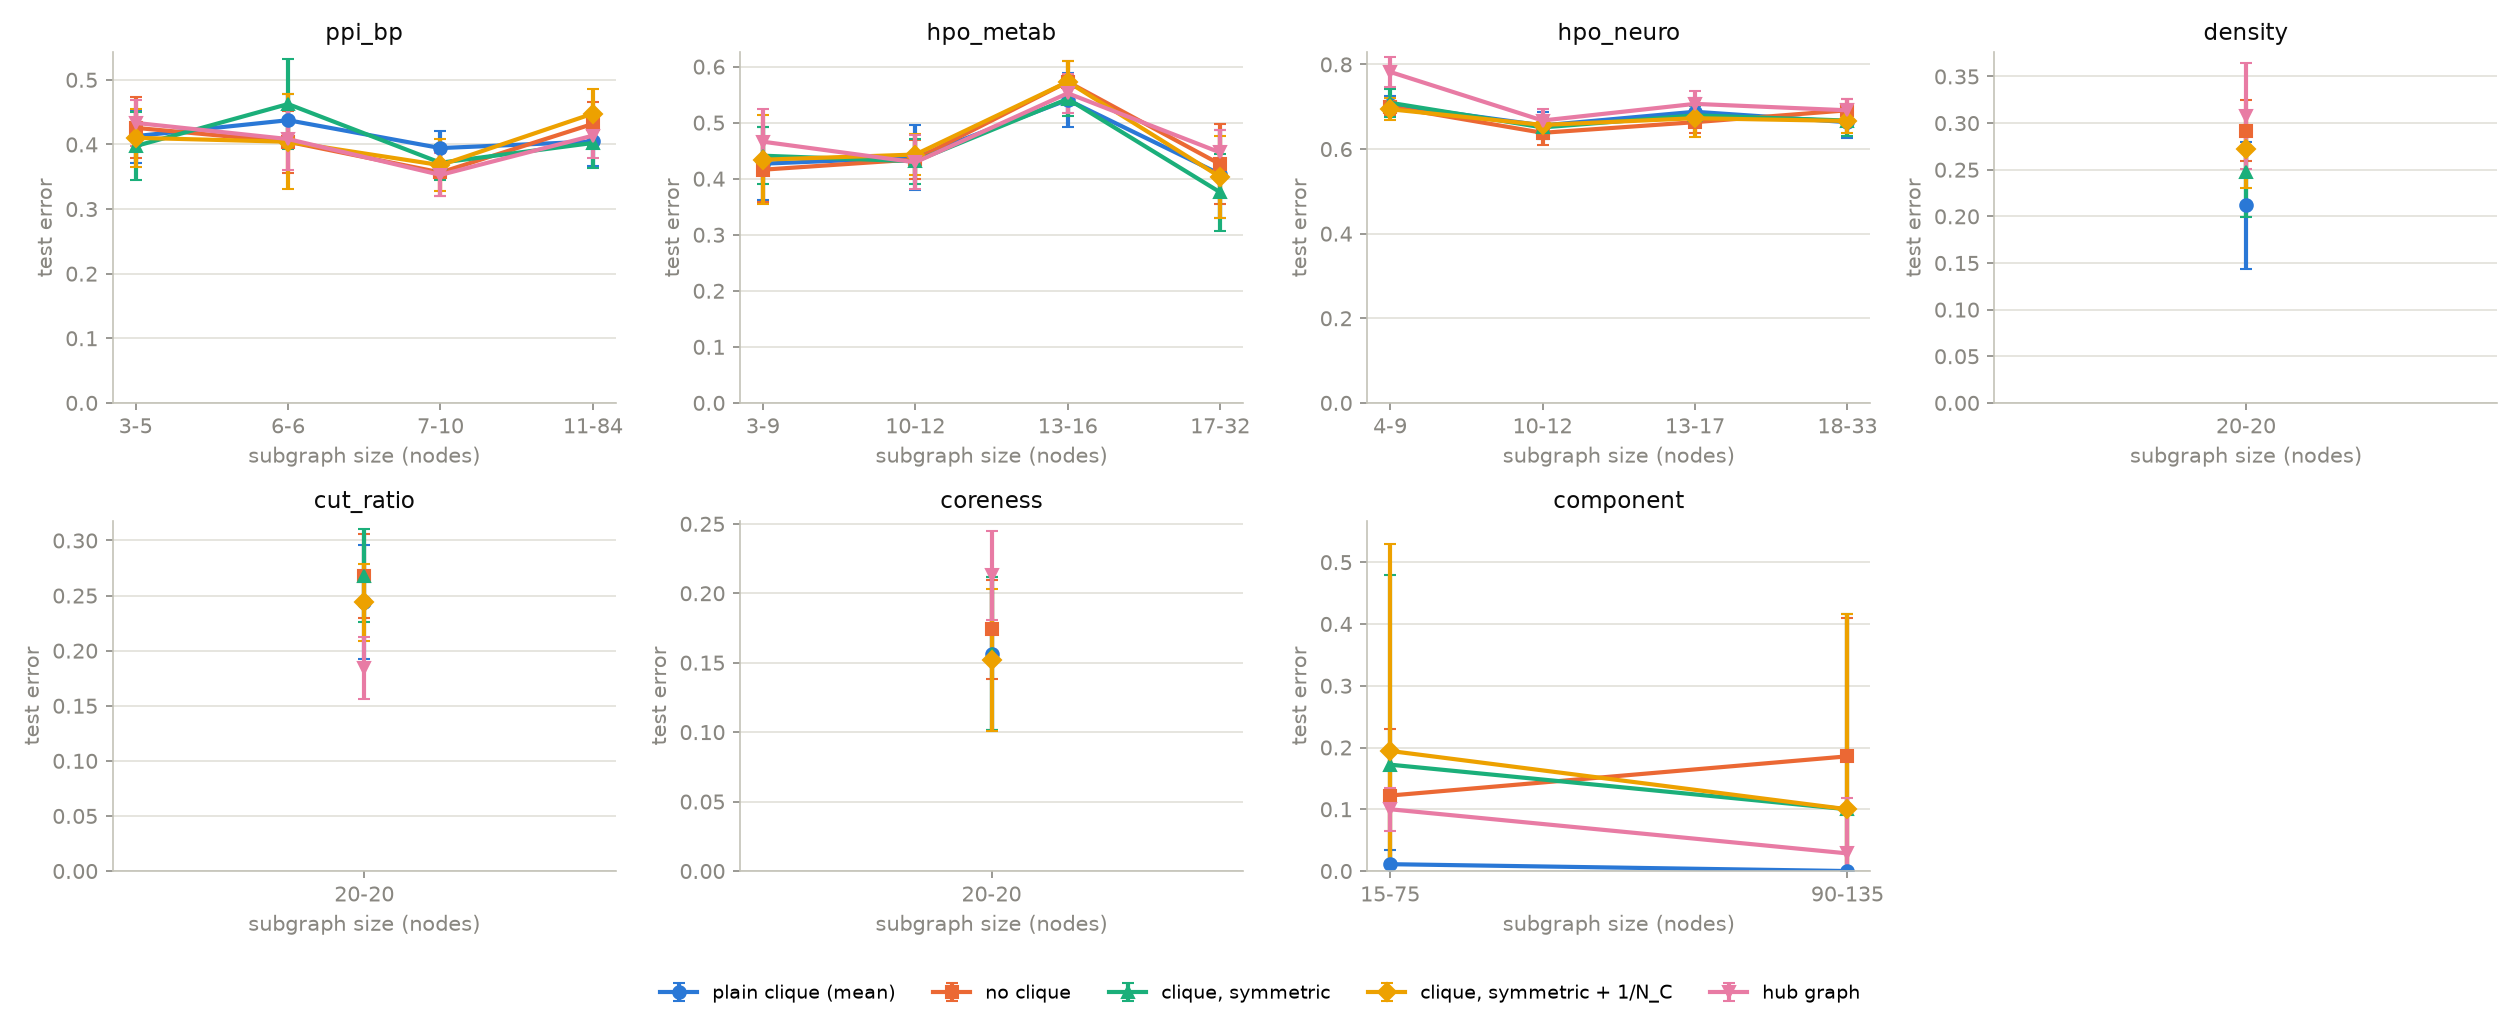
\includegraphics[width=\textwidth]{figures/08_error_vs_size.png}
\caption{Test error by subgraph size, one line per case. Error is the share of test subgraphs
in the group that got a wrong label, over all 10 seeds; bars are the std across seeds. On
hpo\_neuro, where a subgraph can have several labels, ``wrong'' means the predicted label set is
not exactly the true one, so its error is much higher than $1-$F1. density, cut\_ratio and
coreness have only one point because all their subgraphs have 20 nodes.}
\label{fig:size}
\end{figure}

\section*{Next steps}

\paragraph{Where we fall behind.} We are close to GPEN on coreness and component, and far
behind on hpo\_metab, hpo\_neuro, density and cut\_ratio. These four are also the datasets where
subgraphs share nodes: the share of subgraph pairs with at least one node in common is 0\% on
coreness and component and 2\% on ppi\_bp, against 8\% on cut\_ratio and 41--44\% on
hpo\_metab, hpo\_neuro and density (measured on the local data). This is only a match between
two lists; the GLASS paper below suggests it is not the main cause.

\paragraph{What the GLASS paper shows.} GLASS marks each node as inside or outside the
subgraph. To save time it does not do this for one subgraph at a time: it marks a whole batch
at once, and a node counts as inside if it is in any subgraph of the batch. So in GLASS too, a
node in two subgraphs gets one vector per batch. The authors report that this overlap has little
effect. They also report a plain GNN with no marks at all (Table~\ref{tab:plain}).

\begin{table}[H]
\centering
\small
\begin{tabular}{lccccccc}
\toprule
 & ppi\_bp & hpo\_metab & hpo\_neuro & density & cut\_ratio & coreness & component \\
\midrule
plain GNN (no marks) & 61.3 & 59.7 & 66.8 & 46.2 & 88.7 & 53.6 & 99.8 \\
GLASS                & 61.9 & 61.4 & 68.5 & 93.0 & 93.5 & 84.0 & 100.0 \\
our best             & 60.6 & 55.3 & 63.2 & 78.8 & 81.6 & 84.8 & 99.2 \\
\bottomrule
\end{tabular}
\caption{Test micro-F1 ($\times 100$). The first two rows are from Tables 5 and 6 of the GLASS
paper (10 seeds); ``our best'' is the best of our six models in Table~\ref{tab:results}.}
\label{tab:plain}
\end{table}

\paragraph{On hpo, even a plain GNN beats us.} Without any marks, GLASS's plain GNN gets 59.7 on
hpo\_metab and 66.8 on hpo\_neuro, 4.4 and 3.6 points above our best. So the gap there is not
about marking nodes or about overlap. One clear difference is the input: GLASS starts from node
vectors pretrained on link prediction, while our best runs learn their own vectors, which
overfit (train F1 near 1.0). But in our search the pretrained SubGNN vectors did much worse
than learned ones (best test 46.4 on hpo\_metab and 49.9 on hpo\_neuro, from about 20 trials
each). So the cause on hpo is still open.

\paragraph{On density, the marks matter.} The plain GNN gets 46.2 and GLASS 93.0. Density is
the number of graph edges inside the subgraph out of all possible pairs, so the model has to
know which edges stay inside. Our structural input gives each node its number of neighbors that
are in any of its subgraphs, which is wrong for a node in two subgraphs, and RGCN takes a mean
over neighbors, so it cannot count edges by itself.

\paragraph{On cut\_ratio, we are below the plain GNN} (81.6 against 88.7), so something more
basic is missing there.

\paragraph{What we will try.}
\begin{itemize}[itemsep=2pt]
  \item \textbf{Counts on the hub.} Each hub belongs to exactly one subgraph, so it can hold that
        subgraph's own counts: its number of nodes, of graph edges inside it, and of graph edges
        leaving it. These go in as input features of the hub. On density and cut\_ratio these
        three numbers almost give the label away, so a gain there would not show much.
  \item \textbf{Rebuild GLASS's plain GNN in our code.} Our backbone with no subgraph edges and
        pretrained input should reach about 60 on hpo\_metab. If it does not, the gap is in our
        training or input, not in the model.
  \item \textbf{A check on overlap.} Plot test error against how many other subgraphs a test
        subgraph shares nodes with, from the saved predictions. If error does not rise, overlap
        can be dropped as a cause.
\end{itemize}

\end{document}
